\chapter{静电场}
\setcounter{example_counter}{1}

\section{电场强度}

\subsection{电荷的基本知识}

\subsubsection{电荷的性质}

\begin{itemize}
    \item 种类：电荷分为正、负两种，同性相斥、异性相吸
    \item 量子性：所有电荷都是元电荷$e=\SI{1.6e-19}{C}$的整数倍
    \item 电荷守恒：封闭系统的正负电荷的电量代数和保持不变
\end{itemize}

若带电体的尺度远小于研究问题，可视为\textbf{点电荷}，是一种理想模型。

\subsubsection{库仑定律}

\noindent
\begin{minipage}{0.74\linewidth}
\setlength{\parindent}{2em}
\setlength{\parskip}{0.5em}
\linespread{1.3}

真空中两个静止点电荷的作用力，与他们所带电量的乘积成正比，与距离的平方成反比，作用力的方向沿着他们的连线。

同种电荷相互吸引，异种电荷相互排斥。

\begin{formula}
    $\vec{F}=\dfrac{q_1q_2}{4\pi\varepsilon_0 r^2}\vec{e}$
\end{formula}

其中，$\varepsilon_0=\dfrac{1}{4\pi k}=\SI{8.85e-12}{C^2/(N\cdot m^2)}$称为真空介电常量。

\end{minipage}
\hfill
\begin{minipage}{0.25\textwidth}
    \vspace{-1em}
    \centering 
\includegraphics[width=\textwidth]{asset/ch7/T2.png}
\end{minipage}

\note{这与高中所学$F=k\dfrac{q_1q_2}{r^2}$的形式相同，一些教材将其形式记为$\vec{F}=\dfrac{q_1q_2}{4\pi\varepsilon_0 r^3}\vec{r}$，本质上也相同。}

\subsubsection{电力的叠加原理}

两个点电荷之间的作用力，不因第三个点电荷的存在而改变。

\subsection{电场强度}

若试探电荷$q$在电场中受力为$\vec{F}$，定义电场强度为

\begin{formula}
    $\vec{E}=\dfrac{\vec{F}}{q}$
\end{formula}

\note{电场强度是矢量，方向为正电荷受力的方向，单位为$\unit{N/C}$或$\unit{V/m}$.}

\warn{注意电场强度是电场本身的性质，与试探电荷无关。}

若已知电场强度的空间分布，则电荷$q$的受力为$\vec{F}=q\vec{E}$

\subsection{电场强度的计算}

\subsubsection{点电荷产生的电场}

\noindent
\begin{minipage}{0.75\linewidth}
\setlength{\parindent}{2em}
\setlength{\parskip}{0.5em}
\linespread{1.3}

根据电场强度的定义，点电荷产生的电场强度为

\begin{formula}
    $\vec{E}=\dfrac{q}{4\pi \varepsilon_0 r^2}\vec{e}_r=\dfrac{kq}{r^2}\vec{e}_r$
\end{formula}

\end{minipage}
\hfill
\begin{minipage}{0.23\textwidth}
    \vspace{-1em}
    \centering 
\includegraphics[width=\textwidth]{asset/ch7/T1.png}
\end{minipage}

\subsubsection{点电荷系产生的电场}

多个点电荷产生的电场，可使用\textbf{电场强度叠加原理}进行叠加计算。

电场中任一点处的总电场强度，等于各个点电荷单独存在时，在该点所产生的电场强度的矢量和。

\begin{example}{叠加法求场强}
    一根不导电的细塑料杆，$Q=\SI{3.12e-9}{C}$的正电荷均匀分布在杆上。现将塑料杆弯成近乎完整的圆，半径$R=\SI{0.5}{m}$，杆的两端有$d=\SI{2}{cm}$的缝隙，求圆心处的电场强度。
    \tcblower
    原带电体可以视为一个完整的圆和缺口处的一个点电荷的叠加。

    \vspace{-0.8em}

    \begin{center}
        
\includegraphics[width=0.4\textwidth]{asset/ch7/T3.png}
    \end{center}

    \vspace{-0.8em}
    
    而完整的圆在圆心处产生的电场为零，所以只需考虑点电荷产生的电场。

    \vspace{0.5em}

    应补充的点电荷的电量为$q=Q\cdot \dfrac{d}{2\pi R-d}=\SI{2.0}{C}$

    \vspace{0.6em}

    电场强度的大小为$E=\dfrac{q}{4\pi\varepsilon_0 R^2}=\SI{0.72}{V/m}$，方向指向缝隙。
    
    \tcbline

    \vspace{-0.5em}
    
    \begin{minipage}{0.82\linewidth}

    【补充练习】在边长为$\SI{1}{m}$的正方体的八个顶点上，各有一个电荷量为$\SI{1e-6}{C}$的电荷，其中七个是正电荷，一个是负电荷。求正方体中心处的电场强度。
    
    \end{minipage}
    \hfill
    \begin{minipage}{0.15\textwidth}
        %\vspace{-1em}
        \centering 
\includegraphics[width=\textwidth]{asset/ch7/T4.png}
    \end{minipage}
    
\end{example}

\subsubsection{连续型物体的场强}

对于均匀带电的连续体，可先设出单位长度/面积/体积的电荷密度，切分成小段之后，每个微元都可视为一个点电荷，再利用积分叠加求解。
电荷分布若有对称性，某个方向也许无需计算，从而简化求解。

%\vspace{-1em}

%\begin{center}
%    
\includegraphics[width=0.8\textwidth]{asset/ch7/T5.png}
%\end{center}

\begin{example}{利用积分计算场强：线型}
    长为$L=\SI{0.2}{m}$的直线AB上均匀分布着$Q=\SI{8e-8}{C}$正电荷，以中点O为原点。(1) 对于AB延长线上的点P$(x)~(x>0.1)$，求P点的场强；(2) 相同的带电直线CD放在AB延长线上，两者相距$L=\SI{0.2}{m}$，求他们之间的作用力。



    \centering 
\includegraphics[width=0.4\textwidth]{asset/ch7/T6.png}

    \vspace{-0.5em}
    
    \tcblower
    (1)~线电荷密度$\lambda=\dfrac{Q}{L}=\SI{4e-7}{C/m}$，将直线AB切分成长度为$dl$的小段，每段电荷量为$\lambda dl$.

    \vspace{0.3em}

    在直线AB上，取坐标为$l$的小段（$-0.1<l<0.1$），它在P$(x)$处产生的电场强度方向为$+x$.

    \vspace{0.3em}
    
    大小为$dE=\dfrac{\lambda dl}{4\pi\varepsilon_0 (x-l)^2}$，方向为$+x$. （注意积分变量是$l$，$x$视为常数）

    \vspace{0.3em}

    直线AB在P点的场强是$\displaystyle\int_{-L/2}^{L/2}{\dfrac{\lambda dl}{4\pi\varepsilon_0 (x-l)^2}}=\left.\dfrac{\lambda}{4\pi\varepsilon_0 (x-l)}\right|_{-L/2}^{L/2}=\dfrac{720}{x^2-0.01}$(SI)，方向为$+x$

    \vspace{0.3em}

    (2)~直线CD也切分成长度为$dx$的小段，每段电荷量为$dq=\lambda dx$.

    \vspace{0.3em}

    坐标为$x$处的小段（$0.3<x<0.4$）受力大小为$dF=E\cdot dq=\dfrac{720\lambda dx}{x^2-0.01}$，方向为$+x$

    \vspace{0.3em}

    直线CD受力大小为$F=\displaystyle\int_{0.3}^{0.5}{\dfrac{720\lambda dx}{x^2-0.01}}=1.44\times10^{-3} \left.\ln{\dfrac{x-0.1}{x+0.1}}\right|_{0.3}^{0.5}\approx \SI{4.1e-4}{N}$，方向为$+x$
    
    \tcbline
    【补充练习】用带电细线弯成半径为$R$的半圆，在以下情况下求圆心处的场强。
    
    (1)~细线均匀带电，总电荷量为$+2Q$；(2)~左半部分均匀分布电荷$+Q$，右半部分均匀分布电荷$-Q$

    \centering 
\includegraphics[width=0.45\textwidth]{asset/ch7/T7.png}

    \vspace{-0.5em}
\end{example}

\begin{example}{利用积分计算场强：面型}
    求下列均匀带电体，通过圆心的轴线上各点的电场强度。
    
    (1) 半径为$R$的环形细线，线电荷密度为$\lambda$；(2) 半径为$R$的圆盘，面电荷密度为$\sigma$

    \vspace{-0.8em}
    
    \begin{center}
        
\includegraphics[width=0.3\textwidth]{asset/ch7/T8.png}
        
\includegraphics[width=0.25\textwidth]{asset/ch7/T9.png}
    \end{center}

    \vspace{-1.5em}    
    
    \tcblower
    
    (1)~根据对称性，对于轴线上各点，电场强度一定只有$x$分量，$y,z$分量抵消为零。

    下面考虑$x>0$的情况，对于$x<0$的情况，电场强度相互对称，无需另行求解。

    将环形细线切成圆心角为$d\theta$的小段，每段长度为$Rd\theta$，电荷量为$R\lambda d\theta$

    \vspace{-0.3em}

    这个小段到轴线上坐标为$x$点的距离为$\sqrt{R^2+x^2}$,它产生的电场强度大小为$\dfrac{R\lambda d\theta}{4\pi\varepsilon_0 (R^2+x^2)}$

    但根据对称性的分析，只取$x$分量，这个分量为$\dfrac{R\lambda x d\theta}{4\pi\varepsilon_0 (R^2+x^2)^{\frac{3}{2}}}$

    \vspace{0.3em}

    \note{注意这个式子当中$x$是常数，积分变量是$\theta$}

    \vspace{0.5em}

    整个环产生的电场强度为$\dfrac{R\lambda x}{4\pi\varepsilon_0 (R^2+x^2)^{\frac{3}{2}}}\displaystyle\int_0^{2\pi}{d\theta}=\dfrac{R\lambda x}{2\varepsilon_0 (R^2+x^2)^{\frac{3}{2}}}$，方向沿轴线远离圆环。

    (2)~仍然根据对称性可知，电场强度只有$x$分量，且只需考虑$x>0$的情况。
    
    圆盘可视为无数个圆环的叠加，将其切分为宽度均为$dr$的圆环，每个圆环的线电荷密度为$\sigma dr$

    \vspace{0.5em}

    对于半径为$r$的圆环，产生的场强为$\dfrac{rx\sigma dr}{2\varepsilon_0 (r^2+x^2)^{\frac{3}{2}}}$，方向沿轴线远离圆盘。

    因此整个圆盘产生的电场强度为$\displaystyle\int_0^R\dfrac{rx\sigma dr}{2\varepsilon_0 (r^2+x^2)^{\frac{3}{2}}}=-\dfrac{x\sigma}{2\varepsilon_0}\left.\dfrac{1}{\sqrt{r^2+x^2}}\right|_0^R=\dfrac{\sigma}{2\varepsilon_0}\left(1-\dfrac{x}{\sqrt{x^2+R^2}}\right)$
    
    \tcbline
    【补充练习】半径为$R$的均匀带电半球面，面电荷密度为$+\sigma$，求球心处的电场强度。
\end{example}

\section{高斯定理}

\subsection{电场线}

\noindent
\begin{minipage}{0.68\linewidth}
\setlength{\parindent}{2em}
\setlength{\parskip}{0.5em}
\linespread{1.3}

电场可用电场线直观表示，在图中：
\begin{itemize}
    \item 电场线从正电荷（或无穷远）出发，到负电荷（或无穷远）结束
    \item 电场线不会相切或相交
    \item 电场线的疏密程度表示场强的大小，切线方向表示场强的方向
\end{itemize}

\end{minipage}
\hfill
\begin{minipage}{0.3\textwidth}
    \vspace{-1em}
    \centering 
\includegraphics[width=\textwidth]{asset/ch7/T10.png}
\end{minipage}

\subsection{电通量}

在电场中，穿过一个面的电通量$\Phi_e$是场强对面积$S$的面积分，可以理解为有几条电场线穿过这个面。

\begin{formula}
    $\Phi_e=\displaystyle\iint_S\vec{E}\cdot d\vec{S}$
\end{formula}

\note{电通量是标量，但需要区分电场线是从哪个方向穿过这个面的，对于一个封闭曲面，可以想象成“穿进去”和“穿出来”的区别。如果先穿进去，又穿出来，相当于没有作用。}

对于匀强电场而言，可以直接用电场强度的大小，乘以垂直于这个方向的面积。

\vspace{-1.2em}

\begin{center}
    
\includegraphics[width=0.3\textwidth]{asset/ch7/T13.png}
\end{center}

\vspace{-1.5em}

\begin{example}{求电通量}
    在匀强电场$E$中，有一个半径为$R$的无底半球面。在以下情况下求通过半球面的电通量：(1)~底面与电场线垂直；(2)~底面与电场线平行；(3)~电场线与底面的夹角为$30^\circ$

    \vspace{-0.5em}
    
    \begin{center}
        
\includegraphics[width=0.7\textwidth]{asset/ch7/T11.png}
    \end{center}

    \tcblower

    (1)~垂直迎着电场线的面积是$\pi R^2$，因此电通量为$\Phi_e=\pi R^2E$

    (2)~所有电场线都是先进入这个面，又从对面穿出去了，因此电通量为$\Phi_e=0$

    (3)~迎着电场线的面积是$\pi R^2\sin{30^\circ}$，因此电通量为$\Phi_e=\dfrac{1}{2}\pi R^2E$

    \tcbline

    \begin{minipage}{0.85\linewidth}

    【补充练习】在点电荷$+q$的电场中，有一个半径为$R$的圆形平面，电荷与圆心的连线垂直于圆面，且距离也为$R$，求通过此平面的电通量。
    
    \end{minipage}
    \hfill
    \begin{minipage}{0.12\textwidth}
        \centering 
\includegraphics[width=\textwidth]{asset/ch7/T12.png}
    \end{minipage}
    
\end{example}

\subsection{高斯定理的内容}

在真空的静电场内，通过任意封闭曲面的电通量，等于该封闭面所包围的电荷的电量代数和的$\dfrac{1}{\varepsilon_0}$倍，可简化理解为单位正电荷发出$\dfrac{1}{\varepsilon_0}$条电场线。

\begin{formula}
    $\Phi_e=\varoiint_S {\vec{E}\cdot d\vec{S}}=\dfrac{\sum q_{\text{内}}}{\varepsilon_0}$
\end{formula}

只有封闭面内的电荷对$\Phi_e$有贡献，外部的电荷没有贡献。如果面内没有电荷，或正负电荷互相抵消，则电通量为零。

\vspace{-1.2em}

\begin{center}
    
\includegraphics[width=0.8\textwidth]{asset/ch7/T14.png}
\end{center}

\vspace{-1.5em}

\note{在运用高斯定理时，选择的封闭曲面称为高斯面。}

\warn{封闭曲面的电通量为零，不能说明内部没有电荷，也可能正负电荷量相等。}

\begin{example}{高斯定理的概念}
    \begin{minipage}{0.78\linewidth}

    (1)~点电荷在真空中的分布如图所示，S为闭合曲面，求通过该闭合曲面的电通量$\displaystyle\oint_S{\vec{E}\cdot d\vec{S}}$，其中$\vec{E}$是哪些点电荷产生的场强？(2) 若在闭合曲面外部再引入一个电荷，则曲面上的场强是否变化？电通量是否变化？
    
    \end{minipage}
    \hfill
    \begin{minipage}{0.2\textwidth}
        %\vspace{-1em}
        \centering 
\includegraphics[width=\textwidth]{asset/ch7/T15.png}
    \end{minipage}
    
    \tcblower

    (1)~高斯定理中的电通量是由所有电荷产生的，因此是由$q_1\sim q_5$产生的

    (2)~再引入一个电荷，则各处场强都会变化，但外部电荷对封闭曲面的电通量没有影响。
    
    \tcbline
    【补充练习】判断以下说法是否正确：(1)~高斯定理只适用于具有对称性的静电场；(2)~如果高斯面内无电荷，则高斯面上场强处处为零；(3)~若高斯面上场强处处为零，则高斯面内无电荷；(4)~若高斯面上场强处处不为零，则高斯面内一定有电荷；(5)~若高斯面内有净电荷，则通过高斯面的电通量一定不为零。
\end{example}

\begin{example}{利用高斯定理求电通量}
    (1)~在棱长为$L$的正方体中心处，有一个电荷量为$q$的正电荷，求穿过正方体每个面的电通量；(2)~若将这个正电荷放在这个正方体的一个顶点，求穿过正方体每个面的电通量。
    \tcblower
    
    \begin{minipage}{0.83\linewidth}

    (1)~根据高斯定理，整个正方体的电通量$\Phi_e=\dfrac{q}{\varepsilon_0}$

    \vspace{0.5em}

    根据对称性，穿过六个面的电通量应该完全相同

    \vspace{0.5em}
    
    因此穿过各个面的电通量都是$\Phi_e=\dfrac{q}{6\varepsilon_0}$
    
    \end{minipage}
    \hfill
    \begin{minipage}{0.15\textwidth}
        %\vspace{-1em}
        \centering 
\includegraphics[width=\textwidth]{asset/ch7/T16.png}
    \end{minipage}
    
    \begin{minipage}{0.73\linewidth}

    (2)~假想8个相同的立方体堆叠成一个大立方体（棱长为$2L$），点电荷放

    \vspace{0.5em}
    
    在中心。根据上一题结果，穿过各个面的电通量都是$\Phi_e=\dfrac{q}{6\varepsilon_0}$

    \vspace{0.5em}

    要求的立方体位于大立方体的一个角，可以看出有3个面刚好是大立方

    \vspace{0.5em}
    
    体的面的$\dfrac{1}{4}$，这三个面的电通量为$\Phi_e=\dfrac{q}{24\varepsilon_0}$

    \vspace{0.5em}

    另外三个面与电场线平行，并没有电场线穿过它们，因此电通量为零。
    
    \end{minipage}
    \hfill
    \begin{minipage}{0.25\textwidth}
        %\vspace{-1em}
        \centering 
\includegraphics[width=\textwidth]{asset/ch7/T17.png}
    \end{minipage}

    \tcbline
    【补充练习】在空间中存在$+x$方向的电场，$E_x=800\sqrt{x}$（SI），有一个棱长为$\SI{1}{m}$的立方体放在空间中，位置如图所示，求：(1)~通过立方体的电通量；(2)~立方体内的总电荷量。

    \vspace{-1.2em}

    \begin{center}
        
\includegraphics[width=0.3\textwidth]{asset/ch7/T18.png}
    \end{center}

    \vspace{-1.5em}
\end{example}

\section{利用高斯定理求电场强度}

虽然高斯定理适用于任何电场，但利用高斯定理求电场强度时，只能解决具有某种对称性的情况。

\subsection{球对称}

对于球形均匀带电体，电场线的方向一定过球心，取高斯面为半径为$r$的球面。

根据高斯定理，可列出$\Phi_e=\dfrac{\sum q_{\text{内}}}{\varepsilon_0}=E\cdot 4\pi r^2$

\subsubsection{均匀带电球壳}

对于均匀带电球壳，设总电荷量为$Q$，半径为$R$.

\begin{itemize}
    \item 在球壳内部（$r<R$），高斯面内无电荷，场强为零
    \item 在球壳外部（$r\geq R$），高斯面内有所有电荷$Q$，场强等同于将所有电荷集中于球心的点电荷
\end{itemize}


\noindent
\begin{minipage}{0.55\linewidth}
\setlength{\parindent}{2em}
\setlength{\parskip}{0.5em}
\linespread{1.3}
\begin{formula}
    $
    E=\begin{cases}
    	0&		\left( r<R \right)\\[6pt]
    	\dfrac{kQ}{r^2}&		\left( r\geq R \right)\\
    \end{cases}
    $
\end{formula}

\end{minipage}
\hfill
\begin{minipage}{0.4\textwidth}
    
    \centering 
\includegraphics[width=\textwidth]{asset/ch7/T19.png}
\end{minipage}



\subsubsection{均匀带电球体}

对于均匀带电球体，设半径为$R$，体电荷密度为$\rho$，则总电荷$Q=\sigma\cdot \dfrac{4}{3}\pi R^3$

\begin{itemize}
    \item 在球体内部（$r<R$），$q_{\text{内}}=\sigma \cdot \dfrac{4}{3}\pi r^3$，场强等同于将内部电荷集中于球心的点电荷
    \item 在球体外部（$r\geq R$），高斯面内有所有电荷$Q$，场强等同于将所有电荷集中于球心的点电荷
\end{itemize}

\noindent
\begin{minipage}{0.55\linewidth}
\setlength{\parindent}{2em}
\setlength{\parskip}{0.5em}
\linespread{1.3}
\begin{formula}
    $
    E=\begin{cases}
    	\dfrac{\rho r}{3\varepsilon_0}&		\left( r<R \right)\\[12pt]
    	\dfrac{kQ}{r^2}&		\left( r\geq R \right)\\
    \end{cases}
    $
\end{formula}

\end{minipage}
\hfill
\begin{minipage}{0.4\textwidth}
    
    \centering 
\includegraphics[width=\textwidth]{asset/ch7/T20.png}
\end{minipage}

\subsection{柱对称}

若带电体均匀带电，且关于某一轴线对称，则电场线的方向垂直轴线，大小只与到轴线的距离有关。

可取高斯面为高度为$H$、半径为$r$的圆柱面，可列出$\Phi_e=\dfrac{\sum q_{\text{内}}}{\varepsilon_0}=E\cdot 2\pi rH$

\subsubsection{均匀带电直线}

\noindent
\begin{minipage}{0.6\linewidth}
\setlength{\parindent}{2em}
\setlength{\parskip}{0.5em}
\linespread{1.3}
对于无限长均匀带电直线，设线电荷密度为$\lambda$.

高斯面内有长度$H$的所有电荷$q_{\text{内}}=\lambda\cdot H$，可求得电场强度与到轴线的距离的一次方成反比。

\begin{formula}
    $E=\dfrac{2k\lambda}{r}$
\end{formula}

\end{minipage}
\hfill
\begin{minipage}{0.35\textwidth}
    
    \centering 
\includegraphics[width=\textwidth]{asset/ch7/T21.png}
\end{minipage}

\subsubsection{均匀带电圆筒}

对于无限长均匀带电圆筒，设半径为$R$，面电荷密度为$\sigma$，则折合线电荷密度$\lambda=2\pi R\sigma$

\begin{itemize}
    \item 在圆筒内部（$r<R$），高斯面内无电荷，场强为零
    \item 在圆筒外部（$r\geq R$），高斯面内有长度$H$的所有电荷$Q$，场强等同于带电直线
\end{itemize}


\noindent
\begin{minipage}{0.6\linewidth}
\setlength{\parindent}{2em}
\setlength{\parskip}{0.5em}
\linespread{1.3}
\begin{formula}
    $
    E=\begin{cases}
    	0&		\left( r<R \right)\\[6pt]
    	\dfrac{2k\lambda}{r}&		\left( r\geq R \right)\\
    \end{cases}
    $
\end{formula}

\end{minipage}
\hfill
\begin{minipage}{0.35\textwidth}
    
    \centering 
\includegraphics[width=\textwidth]{asset/ch7/T22.png}
\end{minipage}

\subsubsection{均匀带电圆柱}

对于无限长均匀带电圆柱，设半径为$R$，体电荷密度为$\rho$，则折合线电荷密度$\lambda=\pi R^2\sigma$

\begin{itemize}
    \item 在圆柱内部（$r<R$），$q_{\text{内}}=\rho \cdot \pi r^2H$，场强等同于将内部电荷集中为直线
    \item 在圆柱外部（$r\geq R$），高斯面内有长度$H$的所有电荷$Q$，场强等同于带电直线
\end{itemize}

\noindent
\begin{minipage}{0.6\linewidth}
\setlength{\parindent}{2em}
\setlength{\parskip}{0.5em}
\linespread{1.3}
\begin{formula}
    $
    E=\begin{cases}
    	\dfrac{\rho r}{2\varepsilon_0}&		\left( r<R \right)\\[12pt]
    	\dfrac{2k\lambda}{r}&		\left( r\geq R \right)\\
    \end{cases}
    $
\end{formula}

\end{minipage}
\hfill
\begin{minipage}{0.35\textwidth}
    
    \centering 
\includegraphics[width=\textwidth]{asset/ch7/T23.png}
\end{minipage}

\subsection{面对称}

\noindent
\begin{minipage}{0.85\linewidth}
\setlength{\parindent}{2em}
\setlength{\parskip}{0.5em}
\linespread{1.3}

对于均匀带电的无限大平板，设面电荷密度为$\sigma$.

取高斯面为底面积为$S$的柱面，$q_{\text{内}}=\sigma S$，由$\Phi_e=\dfrac{q_{\text{内}}}{\varepsilon_0}=2ES$

可得无限大平板产生的是匀强电场，电场强度如下。

\begin{formula}
    $
    E=\dfrac{\sigma}{2\varepsilon_0}
    $
\end{formula}

\end{minipage}
\hfill
\begin{minipage}{0.12\textwidth}
    
    \centering 
\includegraphics[width=\textwidth]{asset/ch7/T24.png}
\end{minipage}


\begin{example}{利用高斯定理求场强}
    \begin{minipage}{0.73\linewidth}
     一个半径为$R$的球体内部，电荷的体密度为$\rho=kr$，其中$r$为到球心的距离，$k$为常数。(1)~求电场强度的空间分布；(2)~有一长为$R$的均匀带电细线，线电荷密度为$+\lambda$，沿半径方向放置在距球心$2R$到$3R$处，求细线所受的电场力。
    
    \end{minipage}
    \hfill
    \begin{minipage}{0.25\textwidth}
        \centering 
\includegraphics[width=\textwidth]{asset/ch7/T25.png}
    \end{minipage}
   
    \tcblower

    (1)~这个带电体的电荷为球对称分布，可判断任意点的电场强度方向都沿半径方向远离圆心，取半径为$r$的球面为高斯面，利用高斯定理求场强大小。

    对于半径为$r<R$、厚度为$dr$的球壳，其体积为$4\pi r^2dr$，带电量为$4\pi kr^3dr$

    \vspace{0.3em}

    当$r<R$时，可求出高斯面内的电荷总量为$\displaystyle\int_0^r{4\pi kr^3dr}=\pi kr^4$

    \vspace{0.3em}

    利用高斯定理，可得$r<R$处的电场强度大小$E$应满足$4\pi r^2 E=\dfrac{\pi kr^4}{\varepsilon_0}$，得$E=\dfrac{kr^2}{4\varepsilon_0}$

    当$r\geq R$时，高斯面内的电荷总量就是整个球的电荷量，为$\pi kR^4$

    利用高斯定理，可得$r\geq R$处的电场强度大小$E$应满足$4\pi r^2 E=\dfrac{\pi kR^4}{\varepsilon_0}$，得$E=\dfrac{kR^4}{4r^2\varepsilon_0}$

    \vspace{0.3em}

    (2)~对于到球心距离为$x$、长度为$dx$的带电细线，电荷量为$\lambda dx$，它所受的电场力为$\dfrac{kR^4\lambda dx}{4x^2\varepsilon_0}$

    因此整根细线所受的电场力为$F=\dfrac{kR^2}{4\varepsilon_0}\displaystyle\int_{2R}^{3R}{\dfrac{dx}{x^2}}=\dfrac{kR}{24\varepsilon_0}$，方向沿细线远离球心。
    
    \tcbline
    【补充练习】利用高斯定理求电场强度的空间分布：(1)~一个均匀带电的无限长厚圆柱筒，内外半径分别为$R,2R$，体电荷密度为$+\rho$；(2)~一无限大均匀带电厚壁，壁厚为$b$，体电荷密度为$+\rho$.
\end{example}

\subsection{利用已知带电体求场强}

\begin{example}{利用已知带电体求场强：叠加}

    \begin{minipage}{0.8\linewidth}
     有两个相互平行的无限大均匀带电平板A、B，各处电场强度分布如图所示，求两个平面上的电荷面密度。
    
    \end{minipage}
    \hfill
    \begin{minipage}{0.18\textwidth}
        \centering 
\includegraphics[width=\textwidth]{asset/ch7/T26.png}
    \end{minipage}
    
    \tcblower

    均匀带电的无限大平板的场强$E=\dfrac{\sigma}{2\varepsilon_0}$，以向右为正。

    \vspace{0.5em}

    对于B右侧的场强，可列出$E/3=\dfrac{\sigma_A}{2\varepsilon_0}+\dfrac{\sigma_B}{2\varepsilon_0}$，对于A、B中间的场强，可列出$E=\dfrac{\sigma_A}{2\varepsilon_0}-\dfrac{\sigma_B}{2\varepsilon_0}$

    \vspace{0.5em}

    联立两式可解得$\sigma_A=\dfrac{4}{3}\varepsilon_0 E,~\sigma_B=-\dfrac{2}{3}\varepsilon_0 E$
    
    \tcbline
    \begin{minipage}{0.68\linewidth}
     【补充练习】(1)~两个同心均匀带电球壳，内外半径分别为$R_1,R_2$，带电量分别为$+Q_1,+Q_2$，求电场强度的空间分布；(2)~从半径为$R$的球内，挖去一个直径为$R$的球，如图所示。若该形体均匀带电，体电荷密度为$+\rho$，求球心A和相切处B的电场强度。
    
    \end{minipage}
    \hfill
    \begin{minipage}{0.3\textwidth}
        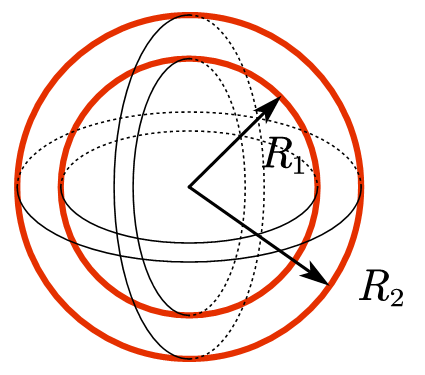
\includegraphics[width=0.5\textwidth]{asset/ch7/T27.png}
        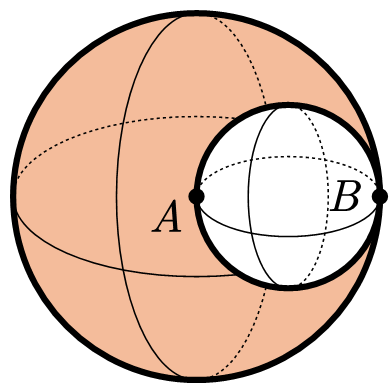
\includegraphics[width=0.45\textwidth]{asset/ch7/T28.png}
    \end{minipage}
    
\end{example}

\begin{example}{利用已知带电体求场强：积分}
    一无限长圆柱面半径为$R$，电荷密度$\sigma=\sigma_0\cos\varphi$（其中$\varphi$为半径与$x$轴的夹角，如下图所示），求圆柱轴线上的场强。
    \tcblower

    根据题意，电荷密度的分布只与$\varphi$有关。若在某处取一窄条（对应圆心角为$d\varphi$），则可视为无限长均匀带电直线，且线电荷密度为$\lambda=\sigma Rd\varphi=\sigma_0 R\cos\varphi d\varphi$

    因为电荷密度的表达式关于$x$轴对称，可以判断场强是$x$方向，只求这一分量即可。

    \vspace{0.5em}

    \begin{minipage}{0.68\linewidth}
     取角度为$\varphi$处的窄条，它在轴线上产生的场强大小为$\dfrac{\sigma_0 R\cos\varphi d\varphi}{2\pi\varepsilon_0 R}$

    在$x$方向上的分量为$-\dfrac{\sigma_0 R\cos^2\varphi d\varphi}{2\pi\varepsilon_0 R}$

    因此整个圆柱面产生的场强为$-\dfrac{\sigma_0}{2\pi\varepsilon_0}\displaystyle\int_0^{2\pi}{ \cos^2\varphi d\varphi}=-\dfrac{\sigma_0}{2\varepsilon_0}$

    这说明场强的大小为$\dfrac{\sigma_0}{2\varepsilon_0}$，方向为$-x$.
    
    \end{minipage}
    \hfill
    \begin{minipage}{0.3\textwidth}
        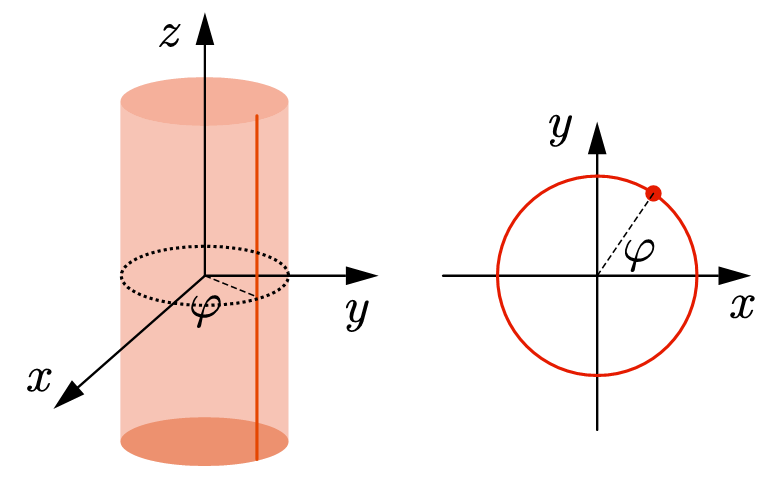
\includegraphics[width=\textwidth]{asset/ch7/T29.png}
    \end{minipage}

    \tcbline
    【补充练习】一个长度无限、宽为$b$的均匀带电平板，电荷面密度为$\sigma=+kx~(0<x<b)$，求薄平板所在平面右侧（$x>b$）的电场分布。
\end{example}

\section{拓展内容}

\subsection{均匀带电直线与圆弧的场强}

\subsubsection{均匀带电圆弧的场强}

\noindent
\begin{minipage}{0.82\linewidth}
\setlength{\parindent}{2em}
\setlength{\parskip}{0.5em}
\linespread{1.3}

对于线电荷密度$\lambda$的均匀带电圆弧，考虑圆心处的场强。

利用对称性，容易判断场强方向一定在圆心角的角平分线上，若圆心角为$2\theta$，可以求出场强大小

\begin{formula}
    $E=\dfrac{2k\lambda}{R}\sin{\theta}$
\end{formula}

\end{minipage}
\hfill
\begin{minipage}{0.15\textwidth}
    
    \centering 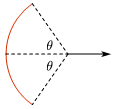
\includegraphics[width=\textwidth]{asset/ch7/T30.png}
\end{minipage}

\subsubsection{均匀带电直线的场强}

均匀带电直线在直线外一点的场强，相当于相同张角的均匀带电圆弧，其半径等于点到直线距离。

\vspace{-1.2em}
\begin{center}
    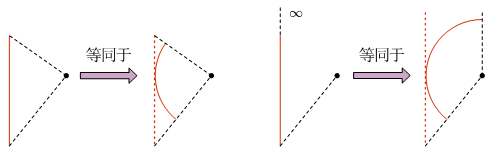
\includegraphics[width=0.6\textwidth]{asset/ch7/T31.png}
\end{center}
\vspace{-1.2em}

\begin{example}{均匀带电直线的场强}
    \begin{minipage}{0.78\linewidth}
     将无限长均匀带电直线弯折成如图所示形状，证明圆心处的场强为零。
    
    \end{minipage}
    \hfill
    \begin{minipage}{0.2\textwidth}
        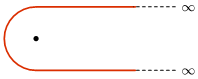
\includegraphics[width=\textwidth]{asset/ch7/T32.png}
    \end{minipage}
    
    \tcblower

    设线电荷密度为$\lambda$，半径为$R$，首先求半圆部分的场强。

    将半圆切分成圆心角$d\theta$的小段，每一段的电荷量$dq=R\lambda d\theta$

    \vspace{0.3em}
    
    在圆心处产生的场强大小为$dE=\dfrac{dq}{4\pi\varepsilon_0 R^2}=\dfrac{\lambda d\theta}{4\pi\varepsilon_0 R}$

    \vspace{0.3em}
    
    以$-x$方向为基准，对于角度为$\theta$的小段，场强的$x$分量大小为$dE_x=\dfrac{\lambda\cos{\theta} d\theta}{4\pi\varepsilon_0 R}$

    \vspace{0.3em}
    
    因此整个半圆的场强大小为$E_1=\displaystyle\int_{-\pi/2}^{\pi/2}\dfrac{\lambda\cos{\theta} d\theta}{4\pi\varepsilon_0 R}=\dfrac{\lambda}{2\pi\varepsilon_0R}$，方向为$+x$

    \vspace{0.3em}
    
    然后求其中一个射线的场强，仍然按照圆心角$d\theta$切小段。

    \vspace{0.3em}

    以$+x$方向为基准，对于角度为$\theta$的小段，$x=\dfrac{R}{\tan\theta}$，两边同时求导得$dx=-\dfrac{Rd\theta}{\sin^2{\theta}}$

    \vspace{0.5em}
    
    所以对于角度为$\theta$的小段，其长度为$dx=\dfrac{Rd\theta}{\sin^2{\theta}}$，电荷量$dq=\dfrac{R\lambda d\theta}{\sin^2{\theta}}$，到圆心距离为$\dfrac{R}{\sin\theta}$

    \vspace{0.3em}
    
    因此它在圆心产生的场强是$dE=\dfrac{dq}{(R/\sin\theta)^2}=\dfrac{\lambda \cdot d\theta}{4\pi\varepsilon_0 R}$，在$x$方向上的分量是$dE_x=\dfrac{\lambda \cos\theta \cdot d\theta}{4\pi\varepsilon_0 R}$

    \vspace{0.5em}
    
    所以一条射线产生的场强的$x$分量为$E_x=\displaystyle\int_0^{\pi/2}\dfrac{\lambda \cos\theta \cdot d\theta}{4\pi\varepsilon_0 R^2}=\dfrac{\lambda}{4\pi\varepsilon_0R}$，方向为$-x$

    \vspace{0.3em}

    根据对称性，另一条射线产生场强的$x$分量也为该值，且$y$分量与之抵消。

    将半圆和射线的$x$分量相加，可得合场强为零。
    
    \tcbline

    \begin{minipage}{0.8\linewidth}
    【补充练习】将无限长均匀带电直线弯折成如图所示形状，线电荷密度为$+\lambda$，求圆心处的场强。
    
    \end{minipage}
    \hfill
    \begin{minipage}{0.18\textwidth}
        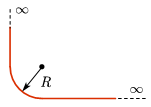
\includegraphics[width=\textwidth]{asset/ch7/T33.png}
    \end{minipage}
\end{example}



